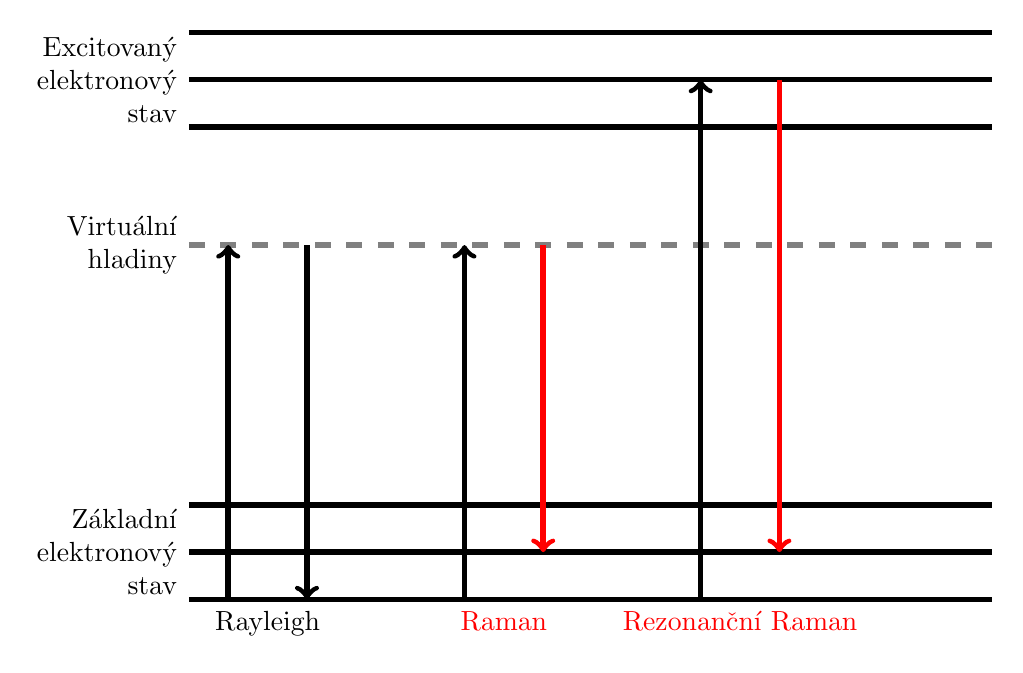
\begin{tikzpicture}[line width=2, scale=1]
	\draw (0,0) -- ++(10.2,0);
	\draw (0,.6) -- ++(10.2,0);
	\draw (0,1.2) -- ++(10.2,0);
	\foreach \x in {0,.4, ...,10}
	{
		\draw [gray] (\x,4.5) -- ++(.2,0);
	}
	\draw (0,6) -- ++(10.2,0);
	\draw (0,6.6) -- ++(10.2,0);
	\draw (0,7.2) -- ++(10.2,0);

	\draw [->] (.5,0) -- ++(0,4.5);
	\draw [->] (1.5,4.5) -- ++(0,-4.5);

	\draw [->] (3.5,0) -- ++(0,4.5);
	\draw [->, color=red] (4.5,4.5) -- ++(0,-3.9);

	\draw [->] (6.5,0) -- ++(0,6.6);
	\draw [->, color=red] (7.5,6.6) -- ++(0,-6);

	\draw(1,0) node [below] {Rayleigh};
	\draw(4,0) node [below] {\textcolor{red}{Raman}};
	\draw(7,0) node [below] {\textcolor{red}{Rezonanční Raman}};
	\draw(0,4.5) node [left, align=right] {Virtuální\\hladiny};
	\draw(0,0.6) node [left, align=right] {Základní\\elektronový\\stav};
	\draw(0,6.6) node [left, align=right] {Excitovaný\\elektronový\\stav};

\end{tikzpicture}
